% Compile with: pdflatex pipeline.tex  (uses tikz, booktabs, listings, hyperref)
\documentclass[11pt]{article}

\usepackage[margin=1in]{geometry}
\usepackage{booktabs}
\usepackage{longtable}
\usepackage{xcolor}
\usepackage{listings}
\usepackage{tikz}
\usetikzlibrary{arrows.meta, positioning, fit, backgrounds, calc}
\usepackage[hidelinks]{hyperref}
\usepackage{enumitem}

\definecolor{codebg}{HTML}{F5F4F0}
\definecolor{accent}{HTML}{1F4E79}
\definecolor{stage}{HTML}{D9EAD3}
\definecolor{artifact}{HTML}{FCE5CD}

\lstset{
  basicstyle=\ttfamily\small,
  backgroundcolor=\color{codebg},
  breaklines=true,
  frame=single,
  rulecolor=\color{lightgray},
  columns=fullflexible,
  showstringspaces=false,
}

\newcommand{\file}[1]{\texttt{#1}}
\newcommand{\mod}[1]{\texttt{#1}}

\title{\textbf{HW/SW Co-Designer:\\ Schematic Generation \& Simulation Pipelines\\ \& System Overview}}
\author{Voltai --- \texttt{SymbolGenAI/test1}}
\date{\today}

\begin{document}
\maketitle

\begin{abstract}
This document describes the end-to-end workflows of the HW/SW Co-Designer. There
are \textbf{two pipelines over one shared source of truth} (the YAML netlists and
per-MPN symbol libraries). The \textbf{generation pipeline}
(\S\ref{sec:overview}--\S\ref{sec:gen-rules}) is a deterministic Python compiler
that turns declarative design intent into a complete, validated Altium schematic
project, gated by a strict connectivity validator and an advisory layout linter;
it is Altium-native end to end (every symbol a committed per-MPN \file{.SchLib})
and runs from one entry point (\texttt{python -m test1.altium.build\_project}).
The \textbf{simulation pipeline} (\S\ref{sec:sim}--\S\ref{sec:sim-lifecycle})
verifies architecture and component values: behavioral SPICE models of testable
sub-circuits (``blocks''), run through \texttt{ngspice}, with AI agents for
datasheet extraction, result interpretation, a bounded iteration loop, and a
SPICE-model lifecycle (generate / update-to-match-schematic / chat-edit). Both
pipelines read the same netlists, so a design change flows into the sims with no
hand-editing. The final section
(\S\ref{sec:gui}) covers the interactive GUI that drives both. (The design was
migrated off an earlier KiCad generator, which has since been removed.)
\end{abstract}

\tableofcontents
\bigskip

%==============================================================================
\section{System overview}\label{sec:overview}
%==============================================================================

The system is a \emph{deterministic compiler} for schematics. Design intent is
expressed once, declaratively, and a chain of pure-Python builders renders it
into Altium-native files. There is no manual drawing step: every wire, pin,
label, and power symbol is emitted programmatically, and every build is checked
by two independent gates --- a strict \textbf{connectivity validator} and an
advisory \textbf{layout linter}.

\begin{description}[leftmargin=1.4em]
  \item[Source of truth (inputs).] Two kinds of input are committed to the repo:
    (1)~\textbf{netlist YAML} (\file{test1/netlist/*.yaml}) describing parts, nets,
    and per-part values; and (2)~\textbf{per-MPN Altium symbol libraries}
    (\file{Parts Library/<MPN>/<MPN>.SchLib}), the committed graphical source of
    truth for every component symbol.
  \item[Builders (processing).] Per-sheet builder modules
    (\mod{build\_power}, \mod{build\_bias}, \dots) place symbols and route nets
    using a common emission API (\mod{shared.AltiumSheet}). A top-level
    orchestrator (\mod{build\_project}) assembles all sheets plus a root sheet
    into one project.
  \item[Outputs (artifacts).] Altium \file{.SchLib} (merged library),
    \file{.SchDoc} (one per sheet), \file{.PrjPcb} (project), and \file{.svg}
    renders for the GUI. SVGs are further converted to PNG for in-agent preview.
  \item[Gates.] \mod{gen.validator} (hard, fails the build on broken
    connectivity) and \mod{altium.layout\_lint} (quality: overlaps, off-grid,
    text globs, centering, \dots).
\end{description}

%==============================================================================
\section{The Altium back-end library (\texttt{altium\_monkey})}
%==============================================================================

Every Altium file the pipeline reads or writes goes through
\mod{altium\_monkey}, a third-party, pure-Python toolkit for Altium files.

\begin{description}[leftmargin=1.4em]
  \item[Where it comes from.] PyPI distribution \texttt{altium-monkey} (import
    name \mod{altium\_monkey}), pinned at \textbf{v2026.5.26}; source repository
    \url{https://github.com/wavenumber-eng/altium_monkey}. It is installed into
    the Altium spike virtual environment
    (\file{c:/Users/mking/Downloads/altium\_spike/.venv}) through which all
    project Python runs, and it requires Python $\geq 3.11,\,<3.13$ (hence the
    spike venv's 3.12).
  \item[What it is.] A dependency-light library that reads and \emph{writes}
    native Altium binary documents (OLE compound files) with \textbf{no Altium
    installation, no Windows COM, and no external CLI}. It covers the schematic
    side we use (\file{.SchLib}, \file{.SchDoc}, \file{.PrjPcb}) as well as PCB
    (\file{.PcbLib}, \file{.PcbDoc}), integrated libraries (\file{.IntLib}), and
    netlist extraction. Crucially it ships an \textbf{in-process SVG renderer}
    (\texttt{to\_svg}), which is what lets the build gate ``does this parse and
    render?'' without launching Altium.
  \item[What it includes.] Three layers: (1)~\emph{document classes}
    (\mod{AltiumSchDoc}, \mod{AltiumSchLib}, \mod{AltiumPrjPcb}, \dots) that own
    a collection of records and serialise to/from disk; (2)~\emph{typed records}
    --- one per primitive (\mod{AltiumSchPin}, \mod{AltiumSchWire},
    \mod{AltiumSchPort}, \mod{AltiumSchPowerPort}, \mod{AltiumSchJunction},
    \dots); and (3)~\emph{\texttt{make\_sch\_*} factory helpers} plus the enums
    and coordinate types that parameterise them. We touch only the schematic
    subset; the entire PCB/IPC-2581/Draftsman surface is unused.
\end{description}

\noindent Table~\ref{tab:monkey} lists the exact API surface the pipeline
consumes. Everything else in the package is ignored.

\begin{longtable}{p{0.30\textwidth} p{0.62\textwidth}}
\caption{The \mod{altium\_monkey} API actually used, and where.}\label{tab:monkey}\\
\toprule
\textbf{Symbol} & \textbf{Role in the pipeline}\\
\midrule
\endfirsthead
\toprule
\textbf{Symbol} & \textbf{Role in the pipeline}\\
\midrule
\endhead
\mod{AltiumSchDoc} & The per-sheet document. \mod{shared.AltiumSheet} wraps one and emits into it via \texttt{.add\_object(\dots)}; \texttt{.to\_svg()} renders the sheet (\mod{render\_svg}).\\
\mod{AltiumSchLib} & Per-MPN symbol library: \texttt{AltiumSchLib(path).get\_symbol(name)} / \texttt{.get\_symbol\_names()} to read committed symbols; \texttt{sym.add\_pin(\dots)} / \texttt{add\_symbol} to author; \texttt{AltiumSchLib.merge(inputs, out, handle\_conflicts="error")} to aggregate; \texttt{symbol\_to\_svg} for per-symbol GUI previews.\\
\mod{AltiumPrjPcb} & Project file: \texttt{create\_minimal} + \texttt{add\_document} + \texttt{save} assemble \file{test1.PrjPcb} (\mod{build\_project}).\\
\texttt{make\_sch\_wire}, \texttt{\_junction}, \texttt{\_port}, \texttt{\_power\_port}, \texttt{\_net\_label}, \texttt{\_no\_erc}, \texttt{\_text\_string} & Schematic-object factories called by \mod{AltiumSheet}'s verbs (\texttt{wire}, \texttt{junction}, \texttt{port}, \texttt{power\_at}, \texttt{net\_label}, \texttt{no\_connect}, \texttt{text}).\\
\texttt{make\_sch\_pin} & Authors pins when building symbols (\mod{author\_symbol}, \mod{author\_mosfets}, \mod{normalize\_passive}, \mod{symbols.\_add\_passive}).\\
\texttt{make\_sch\_sheet\_symbol}, \texttt{\_sheet\_entry}, \texttt{\_sheet\_name}, \texttt{\_file\_name} & Build the hierarchical root sheet (\mod{build\_root}).\\
\mod{PinElectrical}, \mod{PortIOType}, \mod{PortStyle}, \mod{PowerObjectStyle}, \mod{Rotation90} & Enums that set pin electrical type, port I/O direction/style, power-symbol glyph, and 90$^\circ$ pin/symbol orientation.\\
\mod{SchPointMils}, \mod{CoordPoint}, \mod{SchRectMils} & Coordinate/rect types (mils). Note: a power port's \texttt{.location} is a \mod{CoordPoint} (not \mod{SchPointMils}) --- relevant to \mod{auto\_fix\_power}.\\
\mod{ColorValue}, \mod{LineWidth}, \mod{SchFontSpec}, \mod{SchHorizontalAlign}, \mod{TextJustification}, \mod{TextOrientation}, \mod{SheetStyle} & Styling: net/power colours, wire width, fonts, text alignment, and page style.\\
\texttt{altium\_text\_metrics.measure\_text\_width} & Stroke-font text width used by \mod{units.text\_width\_mil} to give every label a real bounding box for the linter.\\
\bottomrule
\end{longtable}

\paragraph{Behaviours we depend on (and gotchas).} The in-process
\texttt{to\_svg()} doubles as a parse gate: a document that cannot be serialised
and rendered fails the build, exactly as \texttt{kicad-cli sch export svg} did on
the old path. Two altium\_monkey-specific quirks are handled in our code: (1)~its
SVG draws every \mod{AltiumSchJunction} as a dot, whereas real Altium drops
redundant junctions --- so our junctions are cosmetic and the linter's
\texttt{redundant\_junction} INFO is expected; and (2)~a power port's
\texttt{.location} is a \mod{CoordPoint}, so \mod{auto\_fix\_power} must relocate
it with \texttt{location.from\_mils(\dots)} rather than assigning a
\mod{SchPointMils}.

%==============================================================================
\section{Pipeline diagram}
%==============================================================================

\begin{figure}[h]
\centering
\resizebox{\textwidth}{!}{%
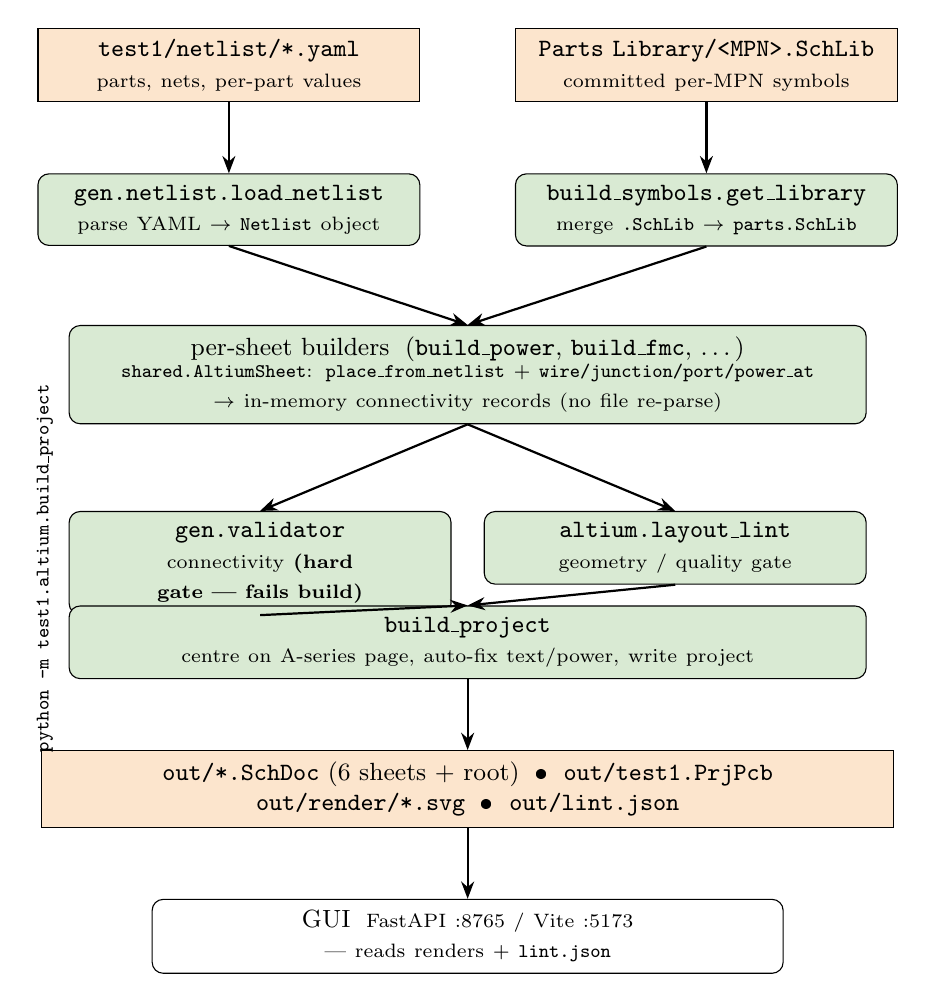
\begin{tikzpicture}[
  font=\small,
  stage/.style={draw, rounded corners, fill=stage, align=center,
                minimum height=2.4em, inner sep=4pt},
  art/.style={draw, fill=artifact, align=center,
              minimum height=2.2em, inner sep=4pt},
  gate/.style={draw, rounded corners, fill=stage, align=center,
               minimum height=2.4em, text width=13em, inner sep=4pt},
  arr/.style={-{Stealth[length=2.2mm]}, thick},
  node distance=9mm and 12mm,
]
% --- inputs on disk ---
\node[art, text width=13em] (yaml)
  {\file{test1/netlist/*.yaml}\\\scriptsize parts, nets, per-part values};
\node[art, text width=13em, right=of yaml] (schlib)
  {\file{Parts Library/<MPN>.SchLib}\\\scriptsize committed per-MPN symbols};

% --- load / merge ---
\node[stage, text width=13em, below=of yaml] (load)
  {\mod{gen.netlist.load\_netlist}\\\scriptsize parse YAML $\to$ \texttt{Netlist} object};
\node[stage, text width=13em, below=of schlib] (merge)
  {\mod{build\_symbols.get\_library}\\\scriptsize merge \file{.SchLib} $\to$ \file{parts.SchLib}};

% --- per-sheet builders (centred under the two input columns) ---
\coordinate (mid) at ($(load.south)!0.5!(merge.south)$);
\node[stage, text width=28em, below=10mm of mid, anchor=north] (build)
  {per-sheet builders \;(\mod{build\_power}, \mod{build\_fmc}, \dots)\\
   \scriptsize \mod{shared.AltiumSheet}: \texttt{place\_from\_netlist} +
   \texttt{wire/junction/port/power\_at}\\
   \scriptsize $\to$ in-memory connectivity records (no file re-parse)};

% --- gates ---
\node[gate, below=11mm of build, xshift=-7.5em] (val)
  {\mod{gen.validator}\\\scriptsize connectivity \textbf{(hard gate --- fails build)}};
\node[gate, below=11mm of build, xshift=7.5em] (lint)
  {\mod{altium.layout\_lint}\\\scriptsize geometry / quality gate};

% --- assemble ---
\node[stage, text width=28em, below=23mm of build] (proj)
  {\mod{build\_project}\\\scriptsize centre on A-series page, auto-fix text/power, write project};

% --- outputs on disk ---
\node[art, text width=30em, below=of proj] (out)
  {\file{out/*.SchDoc} (6 sheets + root) \;\textbullet\; \file{out/test1.PrjPcb}\\
   \file{out/render/*.svg} \;\textbullet\; \file{out/lint.json}};
\node[stage, text width=22em, fill=white, below=of out] (gui)
  {GUI \;\scriptsize FastAPI :8765 / Vite :5173 --- reads renders + \file{lint.json}};

% --- single Python invocation spans load..assemble ---
\node[rotate=90, font=\scriptsize\ttfamily, anchor=south, left=3mm of build] (drv)
  {python -m test1.altium.build\_project};

% --- edges ---
\draw[arr] (yaml) -- (load);
\draw[arr] (schlib) -- (merge);
\draw[arr] (load.south) -- (build.north);
\draw[arr] (merge.south) -- (build.north);
\draw[arr] (build.south) -- (val.north);
\draw[arr] (build.south) -- (lint.north);
\draw[arr] (val.south) -- (proj.north);
\draw[arr] (lint.south) -- (proj.north);
\draw[arr] (proj) -- (out);
\draw[arr] (out) -- (gui);
\end{tikzpicture}%
}
\caption{End-to-end data flow, top to bottom. Orange = file artifact on disk;
green = Python processing stage. A single invocation
(\texttt{python -m test1.altium.build\_project}, rotated label at left) reads the YAML
netlists and the committed \file{.SchLib} symbols, parses the YAML into an
in-memory \texttt{Netlist}, merges the symbol library, builds and routes each
sheet into connectivity records, gates every sheet through the validator (hard)
and the layout linter (quality), then centres and assembles the project. The GUI
consumes the resulting renders and \file{lint.json}.}
\end{figure}

%==============================================================================
\section{Inputs \& ingestion}\label{sec:ingest}
%==============================================================================

Before either pipeline runs, the committed inputs must exist on disk. There are
three input \emph{kinds}, each with a defined format and a defined way it is
\textbf{ingested} into the repo. Ingestion is a one-time, offline step per part;
the build/sim pipelines only ever \emph{read} the committed result.

\subsection{Input file formats}
\begin{description}[leftmargin=1.4em]
  \item[Netlist YAML \textnormal{(\file{test1/netlist/<sheet>.yaml})}.] The
    declarative source of truth, hand-authored (or agent-edited via the GUI
    changelog/apply flow). One file per sheet. Schema (parsed by
    \mod{gen.netlist.load\_netlist} into a typed \texttt{Netlist}): a
    \texttt{parts:} map of \texttt{refdes -> \{lib, value, dnp, \dots\}} and a
    \texttt{nets:} map of \texttt{netname -> [members]}, where each member is a
    \texttt{REFDES.PIN} token (\texttt{parse\_member} handles multi-unit pins).
    Resistor values carry a tolerance tail (e.g.\ \texttt{"5.11k 0.1\%"}); the
    sim value-parser strips it (\mod{sim.design\_extract}). This is the \emph{one}
    file both pipelines read for connectivity and as-built values.
  \item[Per-MPN Altium symbol \textnormal{(\file{Parts Library/<MPN>/<MPN>.SchLib})}.]
    The committed graphical source of truth for a component symbol --- a native
    Altium binary (OLE compound file) read/written through \mod{altium\_monkey}.
    A part directory may also hold \file{<MPN>.PcbLib} (footprint, carried but not
    used by the schematic pipeline), \file{<MPN>.pinspec.json} (see below), and
    the part's datasheet PDF(s).
  \item[Datasheet PDF \textnormal{(\file{Parts Library/<MPN>/*.pdf})}.] Read by
    the AI agents, not the deterministic build. Because the headless environment
    has no poppler, agents do not open the PDF directly: \mod{sim.read\_pdf}
    renders target pages to PNG via PyMuPDF (with a \texttt{--text-only} fast
    path) and the agent reads those.
\end{description}

\subsection{Two ingestion paths to a committed \file{.SchLib}}
A per-MPN symbol enters the library one of two ways. Both end at the same
artifact (\file{Parts Library/<MPN>/<MPN>.SchLib}) that
\mod{build\_symbols.get\_library} later merges.

\begin{description}[leftmargin=1.4em]
  \item[(1) Ultra Librarian import \textnormal{(\file{\_ul\_incoming/install\_ul.py})}.]
    Vendor symbols are obtained as \textbf{Ultra Librarian zips}
    (\file{\_ul\_incoming/ul\_<MPN>.zip}), extracted under \file{\_ul\_incoming/\_x/}.
    For each entry, \mod{install\_ul} finds the \file{.SchLib} (and optional
    \file{.PcbLib}) in the extracted tree, \textbf{validates} it by opening it
    through \texttt{AltiumSchLib.get\_symbol\_names} (a parse gate --- a symbol
    that won't open is rejected), then copies it to
    \file{Parts Library/<dir>/<dir>.SchLib}, backing up any existing project
    symbol to \file{<dir>.SchLib.bak}. A \texttt{MAP} table translates the UL zip
    stem (e.g.\ \texttt{OPA2388IDGKR}, \texttt{TPS7A8401ARGRR}) to the project's
    part-directory name (\texttt{OPA2388}, \texttt{TPS7A8401A}); ambiguous
    multi-file zips are resolved by matching the file stem to the UL name, else
    the largest. The \file{.PcbLib} copy is additive (footprint kept for later
    PCB work; the schematic pipeline ignores it).
  \item[(2) AI symbol generation \textnormal{(GUI Library tab $\to$
    \mod{author\_symbol})}.] When no vendor symbol exists, the GUI's symbol-gen
    agent reads the datasheet and writes a small \textbf{pin specification},
    \file{Parts Library/<MPN>/<MPN>.pinspec.json} --- a JSON schema of
    \texttt{\{mpn, description, reference, properties, units:[\{unit, pins:[\{number,
    name, type, side\}]\}]\}}, where \texttt{type} is an electrical role
    (input/output/power\_in/\dots) and \texttt{side} (left/right/top/bottom) lays
    pins out by function. \mod{author\_symbol} then \emph{deterministically}
    authors \file{<MPN>.SchLib} from that spec (pins via \texttt{make\_sch\_pin},
    body via the standard glyphs of \S\ref{sec:lint}'s neighbour). The pinspec is
    the reviewable, regenerable intermediate; the \file{.SchLib} is the committed
    output.
\end{description}

\paragraph{Normalization \& passives.} Discrete MOSFETs are (re)authored as
proper enhancement devices with an integrated body diode by \mod{author\_mosfets};
passive R/C parts are normalized / auto-authored with standard glyphs by
\mod{normalize\_passive} and \mod{symbols.\_add\_passive}, then merged into the
library as \file{out/lib/\_passives.SchLib}. So whether a symbol arrived by UL
import or AI generation, its body is brought to the same conventional schematic
form before it reaches a sheet.

\paragraph{Historical note.} Symbols originally came from KiCad
\file{.kicad\_sym} and were translated once into committed \file{.SchLib}; that
one-time migration tooling and the KiCad sources have been removed. UL import and
AI generation are the two live ingestion paths today.

%==============================================================================
\section{The file pipeline: read / write / convert}
%==============================================================================

Table~\ref{tab:files} enumerates the concrete files touched at each stage. All
coordinates are in mils on a 100-mil schematic grid; Altium $Y$ grows upward.

\begin{longtable}{p{0.27\textwidth} p{0.12\textwidth} p{0.51\textwidth}}
\caption{Files read, written, and converted by the pipeline.}\label{tab:files}\\
\toprule
\textbf{File / glob} & \textbf{I/O} & \textbf{Role}\\
\midrule
\endfirsthead
\toprule
\textbf{File / glob} & \textbf{I/O} & \textbf{Role}\\
\midrule
\endhead
\file{test1/netlist/*.yaml} & read & Declarative parts/nets/values; loaded by \mod{gen.netlist.load\_netlist}.\\
\file{Parts Library/<MPN>/<MPN>.SchLib} & read & Committed per-part Altium symbol (source of truth). Pins read via \mod{altium.symlib.read\_pins}.\\
\file{<MPN>.pinspec.json} & read/write & Pin specification used to author a symbol with \mod{author\_symbol}; emitted by the GUI's AI symbol-gen flow.\\
\file{out/lib/parts.SchLib} & write & Aggregated library: all per-MPN \file{.SchLib} merged by \mod{build\_symbols.build\_library}.\\
\file{out/lib/\_passives.SchLib} & write & Auto-authored passives (R/C) merged into the library.\\
\file{out/*.SchDoc} & write & One schematic sheet per builder (\texttt{power}, \texttt{bias}, \texttt{bobcat}, \texttt{fmc}, \texttt{connectors}, \texttt{eeprom}) plus \texttt{root}.\\
\file{out/test1.PrjPcb} & write & Altium project referencing the root + 6 child sheets (cross-sheet nets resolve).\\
\file{out/render/*.svg} & write & Per-sheet SVG, produced by \mod{AltiumSheet.render\_svg} (altium\_monkey \texttt{to\_svg}).\\
\file{out/render/\_view\_*.png} & convert & Dev-only raster (\mod{\_render}: SVG\,$\to$\,reportlab PDF\,$\to$\,PyMuPDF PNG) so the agent can inspect layouts (cairo unavailable on Windows).\\
\file{out/lint.json} & write & Structured lint report for THIS build (counts + per-sheet issues), persisted so the GUI checklist survives a backend restart.\\
\bottomrule
\end{longtable}

\paragraph{Migration note.} The symbols originated as KiCad \file{.kicad\_sym}
and were translated once into committed per-MPN \file{.SchLib} files, which are
now the sole graphical source of truth. The KiCad sources, the one-time
migration tooling, and the legacy KiCad generator have all been removed; nothing
on the build path reads \file{.kicad\_sym}.

%==============================================================================
\section{Stage detail}
%==============================================================================

\subsection{Stage 1 --- Symbol library build (\mod{build\_symbols})}
\mod{get\_library()} resolves each part's library id to an authored symbol name
and merges every per-MPN \file{.SchLib} (plus auto-authored passives) into
\file{out/lib/parts.SchLib} via \texttt{AltiumSchLib.merge(\dots,
handle\_conflicts="error")}. Coverage is verified by reading back pins
(\mod{symlib.read\_pins}).

\paragraph{Standard body glyphs.} Symbols are drawn with conventional schematic
shapes, not generic boxes: \mod{glyphs.py} provides a device classifier and
drawers for a capacitor (parallel plates), resistor (US zig-zag), inductor,
diode, MOSFET, and op-amp (triangle); ICs and connectors keep a rectangle. Each
drawer emits only body primitives (\texttt{add\_line/add\_polyline/add\_polygon/
add\_arc}) relative to the pin \emph{hot-spots}; the pins themselves are never
touched, so the electrical connection points --- and therefore every builder's
routing, the validator, and the linter --- are unchanged, and the net always
attaches at the pin end. The discrete MOSFETs are authored as proper enhancement
devices \emph{with an integrated body diode} (substrate arrow and diode oriented
by channel type) by \mod{author\_mosfets}. \mod{glyphs} is wired into both
new-symbol authoring (\mod{author\_symbol}) and passive authoring
(\mod{symbols.\_add\_passive}, \mod{normalize\_passive}), so a body fix in the
library propagates to every sheet on the next build.

\subsection{Stage 2 --- Sheet building (\mod{shared.AltiumSheet})}
Each per-sheet builder receives the merged library and the parsed netlist and
emits primitives through a single high-level API:
\begin{lstlisting}[language=Python]
s = AltiumSheet(name="power", title="...")
U10 = s.place_from_netlist(lib, lmap, nl, "U10", x=5000, y=5000)  # -> {pin: (x,y)}
s.wire(x1, y1, x2, y2)          # orthogonal net segment
s.junction(x, y)                # T-tap dot (cosmetic; T-intersections connect)
s.port(name, x, y, side="auto") # off-sheet port; body auto-placed clear of wire
s.power_at("GND", x, y)         # power symbol (GND down 270deg, rails up 90deg)
s.text("LDO VIN bypass", x, y)  # annotation
\end{lstlisting}
\mod{AltiumSheet} simultaneously accumulates structured records
(\texttt{\_placed}, \texttt{\_wires}, \texttt{\_junctions}, \texttt{\_labels})
that both gates walk without re-parsing the saved file. Every drawn label and
component value carries a rendered \emph{bounding box} so the linter can reason
about text geometry (see \S\ref{sec:lint}).

\paragraph{Ports never impale their wire.} altium\_monkey always draws a port
body extending $+x$ from its anchor. \texttt{port(side="auto")} inspects the wire
already drawn to the connection point and anchors the body on the side
\emph{away} from the net (e.g.\ \texttt{side="left"} puts the body in the left
margin and connects at its right edge). The connectivity record stays at the
exact connection point, so the validator binds the wire endpoint regardless of
which side the body is drawn on. This is why callers draw the wire \emph{before}
the port.

\subsection{Stage 3 --- Connectivity validation (\mod{gen.validator})}
A union-find graph is built from pins, wire endpoints/interiors (T-intersections
auto-connect), and label anchors. Each YAML net is resolved to a connected
component; mismatches (split nets, unknown refdes/pins, missing members) fail the
build. The validator is backend-agnostic: it walks duck-typed connectivity
records (\texttt{\_placed}, \texttt{\_wires}, \texttt{\_junctions},
\texttt{\_labels}), so the same gate runs over any sheet implementation that
exposes them.

\subsection{Stage 4 --- Layout lint (\mod{altium.layout\_lint})}\label{sec:lint}
The linter is the quality gate. It operates on the same duck-typed records and
treats drawn \textbf{text as 2-D boxes}, not points, so it can detect overlaps a
point model misses. Two entry points run on every build:
\mod{lint(sheet)} (per-\file{.SchDoc}) and \mod{lint\_library(path)}
(per-symbol). Rules are declared once in the \texttt{RULES} registry, the single
source of truth shared by the checks, the build report, and the GUI checklist.
\texttt{ERROR} fails the build; \texttt{WARNING}/\texttt{INFO} are advisory.
The full rule set is given in Table~\ref{tab:rules}.

\subsection{Stage 5 --- Centering \& project assembly (\mod{build\_project})}
Layout is offset-invariant for connectivity, so each sheet is built twice: once
to measure its content bounding box, then again with a grid-snapped, clamped
shift that centers the content on the auto-selected A-series page
(\mod{\_build\_centered} / \mod{\_axis\_shift}). The orchestrator then writes
each \file{.SchDoc}, the root sheet, and \file{test1.PrjPcb}, printing a
per-sheet lint summary (\texttt{E/W/I}) plus every \texttt{ERROR}/\texttt{WARNING}
detail line.

\subsection{Stage 6 --- GUI consumption}
The FastAPI backend (port 8765) serves \file{/api/sheets} (render metadata),
\file{/api/png/<sheet>} (rasterized sheet, cache-busted by mtime), and
\file{/api/lint} (parsed issues + the \texttt{RULES} registry imported directly
from \mod{layout\_lint}). The React/Vite frontend (port 5173) "Schematic
Generator" tab renders the schematic and a \emph{Linter checklist}; its
\textbf{Refresh} button re-pulls renders, freshness, and the live rule list, so
the checklist always reflects exactly what the build gates on.

%==============================================================================
\section{Layout linter rule set}\label{sec:gen-rules}
%==============================================================================

\begin{longtable}{p{0.21\textwidth} p{0.10\textwidth} p{0.10\textwidth} p{0.45\textwidth}}
\caption{Rules in the \texttt{RULES} registry (\mod{layout\_lint}).}\label{tab:rules}\\
\toprule
\textbf{Rule} & \textbf{Severity} & \textbf{Scope} & \textbf{What it catches}\\
\midrule
\endfirsthead
\toprule
\textbf{Rule} & \textbf{Severity} & \textbf{Scope} & \textbf{What it catches}\\
\midrule
\endhead
\texttt{off\_grid} & ERROR & sheet & Pin/wire endpoint off the 100-mil grid.\\
\texttt{diagonal\_wire} & ERROR & sheet & Non-orthogonal (diagonal) wire.\\
\texttt{out\_of\_bounds} & ERROR & sheet & Content extends past the sheet border.\\
\texttt{component\_overlap} & ERROR & sheet & Two component pin-boxes overlap.\\
\texttt{power\_orientation} & WARN & sheet & Power port against convention (GND down, rails up).\\
\texttt{visible\_param\_glob} & WARN & sheet & Visible metadata parameter stacks into a glob.\\
\texttt{wire\_through\_label} & WARN & sheet & Port/power hot-spot sits mid-wire.\\
\texttt{power\_straddles\_net} & WARN & sheet & Power/port glyph straddles the net (net runs through it).\\
\texttt{ground\_on\_top} & WARN & sheet & GND symbol above its net instead of at the bottom.\\
\texttt{wire\_through\_body} & WARN & sheet & Net wire crosses a component body.\\
\texttt{off\_center} & WARN & sheet & Content bunched against an edge.\\
\texttt{cramped\_spacing} & WARN & sheet & Two components closer than the readable gap.\\
\texttt{label\_overlap} & WARN & sheet & Two drawn text boxes overlap (glob).\\
\texttt{label\_over\_symbol} & WARN & sheet & A label/port/value text box over a component body.\\
\texttt{label\_symbol\_clearance} & WARN & sheet & A port/text note flush against the true drawn body ($<$50 mil); aligned passive value labels exempt.\\
\texttt{wire\_through\_port} & WARN & sheet & A net wire crosses a port \emph{body}.\\
\texttt{offpage\_text} & WARN & sheet & A drawn box spills past the sheet border.\\
\texttt{wire\_overlap} & WARN & sheet & Collinear same-axis wires overlap (silent short).\\
\texttt{stub\_t\_short} & ERROR & sheet & Power/port glyph on an unrelated wire's interior (Altium auto-junctions a silent short).\\
\texttt{bridged\_drop} & WARN & sheet & Wire interior crosses a third part's pin.\\
\texttt{duplicate\_wire} & INFO & sheet & Identical wire segment drawn twice.\\
\texttt{redundant\_junction} & INFO & sheet & Junction with $<3$ segments / on a pin.\\
\texttt{pin\_name\_overlap} & WARN & library & Symbol body too narrow; opposing pin names collide.\\
\bottomrule
\end{longtable}

%==============================================================================
\section{The simulation pipeline}\label{sec:sim}
%==============================================================================

The simulation layer is the \emph{second} pipeline over the same inputs. Where
generation renders the netlist into a schematic, simulation verifies the
architecture and component values by running behavioral SPICE models of testable
sub-circuits (\textbf{blocks}) through \texttt{ngspice}. Two principles make it
trustworthy:

\begin{description}[leftmargin=1.4em]
  \item[Behavioral, not transcribed.] The decks are \emph{hand-written
    behavioral} models --- they model device \emph{behavior} (regulation, gain,
    droop), not a transistor-level transcription of the schematic. This keeps a
    block's model small and intentional (a part like the op-amp is one
    \texttt{.subckt}, not its gm guts).
  \item[Values from the as-built design.] Although the topology is hand-authored,
    the component \emph{values} (decoupling caps, the bias sense resistor,
    jumpers) are read from the same \file{netlist/*.yaml} the generator consumes,
    via \mod{sim.design\_extract}. A netlist edit therefore flows straight into
    the sim with no hand-editing. Only genuinely \emph{off-sheet} boundary values
    (source impedance, enable timing, downstream load current, the incoming rail
    voltage) and the pass/acceptance criterion are curated, in
    \file{sim/blocks.yaml}.
\end{description}

\subsection{The block catalog (\file{sim/blocks.yaml})}
Each catalog entry is one testable sub-circuit: the netlist sheet it derives
from, the \texttt{sim\_types} that apply (each with a rationale and a concrete
\texttt{pass:} criterion), the device models it needs, the off-sheet boundary
stubs, and a functional \texttt{group}. \mod{sim.catalog} loads it;
\texttt{resolve\_boundaries} merges a block's base boundaries with a sim type's
\texttt{boundary\_overrides}. A block's \texttt{status} is one of
\texttt{implemented} (a deck builder runs it), \texttt{planned} (curated but no
deck yet), or \texttt{not\_simulatable} (no useful SPICE behavior, documented so
the gap is explicit). The functional groups --- \texttt{power\_generation},
\texttt{power\_distribution}, \texttt{analog\_bias}, \texttt{system\_integration},
\texttt{not\_simulatable} --- order and label the Simulation tab's sidebar
(\texttt{SIM\_GROUPS} in \mod{app}). Current blocks: \texttt{ldo\_rail} (LDO +
load switch), \texttt{opa\_bias} (OPA2388 V-to-I loop), four PDN decap banks
(\texttt{vddio/vddd/vdda1/vdda2\_pdn}), the planned \texttt{system\_sequencing},
and the non-simulatable \texttt{eeprom}/\texttt{fmc}/\texttt{connectors}.

\subsection{Deck builders \& the deck-builder contract}
One module per block lives in \file{sim/decks/} (\mod{ldo\_rail}, \mod{opa\_bias},
\mod{pdn}). A conformant deck builder:
\begin{enumerate}[leftmargin=1.6em, itemsep=1pt]
  \item exposes \texttt{build\_deck(*, mode, **kw) -> (deck\_text, trace\_specs)};
  \item reads as-built values from \mod{sim.design\_extract}
    (\texttt{caps\_on\_net}, \texttt{resistor\_value}, \texttt{sense\_resistance},
    \dots) --- never hardcodes a netlist value;
  \item uses the shared device models (\mod{sim.models}) and boundary stubs
    (\mod{sim.stubs}, \texttt{emit\_stub});
  \item provides analyzer fn(s) returning a dict with an
    \texttt{"overall": "OK"|"FAIL"} key, plus a \texttt{refdes\_map()} tying each
    deck element to its netlist refdes (or \texttt{None} for behavioral
    scaffolding: boundary sources, ammeters, DUT-load stubs);
  \item is wired into \mod{sim.service} dispatch (\texttt{run\_block\_sim} +
    \texttt{build\_deck\_text} + \texttt{\_refdes\_map\_for}) and has a
    \file{blocks.yaml} entry;
  \item stamps provenance once it matches the schematic
    (\S\ref{sec:sim-lifecycle}) and verifies the sim runs.
\end{enumerate}

Table~\ref{tab:simmods} maps the \file{sim/} modules.

\begin{longtable}{p{0.27\textwidth} p{0.65\textwidth}}
\caption{The \file{sim/} module map.}\label{tab:simmods}\\
\toprule
\textbf{Module} & \textbf{Role}\\
\midrule
\endfirsthead
\toprule
\textbf{Module} & \textbf{Role}\\
\midrule
\endhead
\mod{blocks.yaml} & Curated block catalog (the library surfaced in the tab).\\
\mod{catalog.py} & Load the catalog; \texttt{resolve\_boundaries} (base + per-sim merge).\\
\mod{catalog\_edit.py} & Surgical, comment-preserving \file{blocks.yaml} edits.\\
\mod{service.py} & GUI-facing dispatch: (block, sim\_type) $\to$ build deck $\to$ run ngspice $\to$ analyze $\to$ JSON (traces, analysis, parsed circuit). \texttt{has\_deck\_builder()} = does a block have a SPICE model.\\
\mod{runner.py} & Invoke \texttt{ngspice -b} on a deck; parse \texttt{.dat} traces.\\
\mod{models.py} & Shared behavioral device models (LDO, switch, op-amp, FET).\\
\mod{stubs.py} & Boundary stubs (\texttt{RailIn}/\texttt{RailOut}/\texttt{DigitalDrive}/\dots); \texttt{emit\_stub}.\\
\mod{design\_extract.py} & The reader of netlist values for the sim layer (value parse w/ tolerance strip, \texttt{caps\_on\_net}, \texttt{resistor\_value}, \texttt{sense\_resistance}, \texttt{sheet\_refdes}).\\
\mod{simconfig.py} & Operating-point \emph{scenario} cache + freshness (\texttt{is\_fresh}).\\
\mod{dscache.py}, \mod{param\_map.py} & Datasheet-derived device params $\to$ ngspice model inputs (\texttt{param\_map.\_MAP} keys the parts that feed models).\\
\mod{circuit.py} & Parse a deck $\to$ \texttt{\{elements, nets, subckts\}} node-graph for the GUI ``SPICE model'' view (refdes-aware; named pins from subckt ports).\\
\mod{deck\_provenance.py} & Per-block netlist \emph{fingerprint} + staleness: \texttt{model\_status} $\in$ \texttt{none|unknown|fresh|stale}.\\
\mod{iterate\_sim.py} & Bounded re-sim CLI for the interpret agent (hard cap 3).\\
\mod{read\_pdf.py} & Render datasheet PDF pages to PNG (PyMuPDF) + \texttt{--text-only} fast path, so agents can read datasheets (the Read tool can't rasterize PDFs here --- no poppler).\\
\bottomrule
\end{longtable}

\subsection{The simulation run workflow}\label{sec:sim-run}
``Run'' in the Simulation tab is a three-stage, \emph{context-first} flow
(parameters are decided \emph{before} the sim runs) wrapped in a bounded feedback
loop. Each AI stage is a \texttt{claude -p} subprocess streamed to the GUI over
SSE.

\begin{figure}[h]
\centering
\resizebox{0.98\textwidth}{!}{%
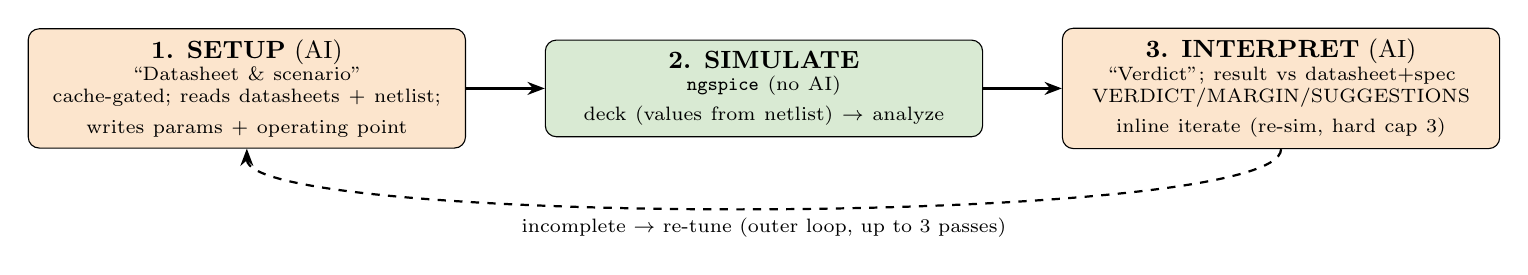
\begin{tikzpicture}[
  font=\small,
  stage/.style={draw, rounded corners, fill=stage, align=center,
                minimum height=2.6em, text width=15em, inner sep=4pt},
  ai/.style={draw, rounded corners, fill=artifact, align=center,
             minimum height=2.6em, text width=15em, inner sep=4pt},
  arr/.style={-{Stealth[length=2.2mm]}, thick},
  node distance=7mm and 10mm,
]
\node[ai] (setup) {\textbf{1. SETUP} (AI)\\\scriptsize ``Datasheet \& scenario''\\\scriptsize cache-gated; reads datasheets + netlist;\\\scriptsize writes params + operating point};
\node[stage, right=of setup] (sim) {\textbf{2. SIMULATE}\\\scriptsize \texttt{ngspice} (no AI)\\\scriptsize deck (values from netlist) $\to$ analyze};
\node[ai, right=of sim] (interp) {\textbf{3. INTERPRET} (AI)\\\scriptsize ``Verdict''; result vs datasheet+spec\\\scriptsize VERDICT/MARGIN/SUGGESTIONS\\\scriptsize inline iterate (re-sim, hard cap 3)};
\draw[arr] (setup) -- (sim);
\draw[arr] (sim) -- (interp);
\draw[arr, dashed] (interp.south) .. controls +(0,-1) and +(0,-1) .. node[below, font=\scriptsize]{incomplete $\to$ re-tune (outer loop, up to 3 passes)} (setup.south);
\end{tikzpicture}%
}
\caption{The simulation run workflow. Orange = AI (\texttt{claude -p}); green =
ngspice. Setup OWNS datasheet $\to$ parameter extraction (cache-gated by
\mod{simconfig.is\_fresh}); the sim runs on the determined operating point;
interpret judges the result against datasheet specs + requirements and may
inline-iterate by correcting a \emph{scenario} parameter and re-running
(\mod{iterate\_sim}, hard-capped at 3). An outer feedback loop re-runs the whole
sequence (up to 3 passes) when a pass comes up incomplete; the tab's workflow
strip shows a green check per completed step and a ``loop $N/3$'' badge.}
\end{figure}

\noindent The endpoints are \texttt{POST /api/sim/setup} (stage 1, returns
\texttt{fresh} or a \texttt{run\_id}), \texttt{POST /api/sim/run} (stage 2,
synchronous), and \texttt{POST /api/sim/interpret} (runs the sim then spawns the
verdict agent). Resilience: the interpret SSE has a watchdog and settles on
error, so a dropped stream or backend restart can't hang the Run; a Cancel button
terminates the live \texttt{claude -p}; persisted state never shows a phantom
``running'' on reload.

%==============================================================================
\section{SPICE-model lifecycle \& agent workflows}\label{sec:sim-lifecycle}
%==============================================================================

A block's deck is \emph{dynamically dependent on the schematic}. Three agents
keep models in sync, and a fourth pair of controls governs which model each agent
runs on. All lifecycle agents share one \texttt{\_DECK\_CONTRACT} (in \mod{agent})
and are \textbf{guarded to the sim layer}: they may write \file{sim/decks/*.py}
and edit \file{sim/blocks.yaml}/\mod{sim.service}, but must \emph{not} touch
\file{netlist/*.yaml}, \file{altium/*}, \file{gen/*}, or the linter --- the
schematic is the \emph{input}, never edited here.

\begin{description}[leftmargin=1.4em]
  \item[Generate (no model).] When a block has no deck builder
    (\texttt{has\_model = false}, \texttt{model\_status = none}),
    \texttt{POST /api/sim/generate-model} $\to$ \mod{start\_sim\_generate\_model}.
    The agent reads the netlist + datasheets, studies the existing decks as
    templates, \emph{writes} \file{sim/decks/<block>.py} + the service dispatch +
    a \file{blocks.yaml} entry, stamps provenance, and verifies the sim runs. The
    GUI shows a \emph{Generate SPICE model} button.
  \item[Update (stale).] When the netlist has changed under a model
    (\texttt{model\_status = stale}), \texttt{POST /api/sim/update-model} $\to$
    \mod{start\_sim\_update\_model}. The agent diffs the current netlist against
    the deck's assumptions, makes the minimal changes to re-sync, re-stamps, and
    verifies. The GUI shows an \emph{Update to match schematic} button. Staleness
    is decided by \mod{sim.deck\_provenance}: a content fingerprint of the block's
    netlist sheet(s) is stamped when a model is generated/updated; if the live
    fingerprint differs, the model is stale.
  \item[Chat-edit (foundation).] \texttt{POST /api/sim/chat-edit} $\to$
    \mod{start\_sim\_chat\_edit} applies a natural-language request to a block's
    pass criteria / boundary params / model / functions (smallest change;
    \texttt{CLARIFY} if ambiguous). The agent and endpoint are wired so the
    interactive chat UI --- gated on a forthcoming chat API --- is a thin
    wire-up, not new machinery.
\end{description}

\paragraph{Per-agent model selection.} Each sim agent \emph{kind} runs on a
selectable Claude model (\texttt{opus}/\texttt{sonnet}/\texttt{haiku}),
overridable from the GUI (the ``Agent models'' control) and persisted in
\file{gui/state/agent\_models.json}. \mod{agent.model\_for(kind)} resolves the
choice per spawn (override $\to$ per-kind default $\to$ global \texttt{MODEL}) and
threads it into \texttt{\_spawn\_claude}; \texttt{GET/POST /api/sim/agent-models}
read and set it. Defaults: the heavy model-authoring agents
(\texttt{sim\_generate}, \texttt{sim\_update}) default to \texttt{opus}; the
extraction/verdict/chat agents to \texttt{sonnet}.

\paragraph{Agent mechanics.} Agents are \texttt{claude -p} subprocesses
(stream-json, \texttt{--permission-mode acceptEdits}, \texttt{cwd=test1/},
reusing the user's \texttt{claude} auth --- no API key). The spike venv's
\texttt{python} dir is prepended to the agent \texttt{PATH} (so a plain
\texttt{python sim/read\_pdf.py} resolves to the PyMuPDF-having interpreter) and
\texttt{PYTHONUTF8=1} is set. Tool allow-lists are sim-scoped; sim agents
auto-discover \file{test1/.claude/skills/} (e.g.\ \texttt{sim-datasheet-extraction}).
Datasheet extraction is a \emph{setup-only} (design-input) step; interpret is
read-only on the param cache.

%==============================================================================
\section{The GUI}\label{sec:gui}
%==============================================================================

The GUI drives both pipelines. The FastAPI backend (port 8765) and the
React/Vite frontend (port 5173) read the same artifacts the build writes. Tabs:
\textbf{Resources} (datasheets / requirements / skills), \textbf{Library}
(per-MPN symbols; AI symbol-gen from a datasheet), \textbf{Generator} (run the
generation pipeline; the linter checklist), \textbf{Simulation} (the whole
simulation pipeline above), and \textbf{Review} (design-review findings + fix
queue). The Simulation panel stays \emph{mounted} across tab switches (hidden via
CSS), so a running sim's loop and SSE subscriptions survive navigating away.

\begin{longtable}{p{0.34\textwidth} p{0.58\textwidth}}
\caption{Key Simulation-tab endpoints (\mod{gui.backend.app}).}\label{tab:simapi}\\
\toprule
\textbf{Endpoint} & \textbf{Role}\\
\midrule
\endfirsthead
\toprule
\textbf{Endpoint} & \textbf{Role}\\
\midrule
\endhead
\texttt{GET /api/sim/blocks} & Catalog + groups + \texttt{has\_model}/\texttt{model\_status}.\\
\texttt{GET /api/sim/circuit} & Parsed deck node-graph (no ngspice) for the ``SPICE model'' view.\\
\texttt{GET /api/sim/simulated-region} & Which sheets/refdes a block covers (cross-sheet highlight).\\
\texttt{POST /api/sim/run} & Run ngspice for one (block, sim\_type).\\
\texttt{POST /api/sim/setup} & Stage 1 (cache-gated) agent.\\
\texttt{POST /api/sim/interpret} & Run + stage 3 (verdict) agent.\\
\texttt{POST /api/sim/generate-model} & Author a new SPICE model (agent).\\
\texttt{POST /api/sim/update-model} & Re-sync a stale model (agent).\\
\texttt{POST /api/sim/chat-edit} & NL edit of a block's sim (agent; foundation).\\
\texttt{GET/POST /api/sim/agent-models} & Per-agent model selection.\\
\texttt{GET/POST /api/sim/requirements} & Edit pass criteria + boundary params.\\
\texttt{POST /api/sim/cache/clear} & Drop scenario / params / counters per block.\\
\texttt{POST /api/agent/\{run\_id\}/cancel} & Terminate a live \texttt{claude -p}.\\
\texttt{GET /api/agent/\{run\_id\}/stream} & SSE of an agent run.\\
\bottomrule
\end{longtable}

%==============================================================================
\section{Reproducing a build / running a sim}
%==============================================================================

\begin{lstlisting}[language=bash]
# All Python runs through the Altium spike venv (Windows):
PY=c:/Users/mking/Downloads/altium_spike/.venv/Scripts/python.exe

# --- Generation pipeline ---
# Full project: merge symbols, build+validate+lint 6 sheets, assemble .PrjPcb
$PY -m test1.altium.build_project
# Lint only, across all sheets:
$PY -m test1.altium.layout_lint
# Dev render a sheet to PNG (SVG -> PDF -> PNG):
$PY -m test1.altium._render power

# --- Simulation pipeline ---
# Run one block/sim_type headlessly (status should be 'ran', or 'no_simulator'):
$PY -c "import sys; sys.path.insert(0,'.'); from test1.sim import service; \
        print(service.run_block_sim('ldo_rail','dc_op_point')['status'])"
# Model-vs-schematic status / stamp the netlist fingerprint:
$PY test1/sim/deck_provenance.py --status ldo_rail
$PY test1/sim/deck_provenance.py --stamp  ldo_rail

# --- GUI (drives both pipelines) ---
# backend (repo root on PYTHONPATH):  cd test1/gui/backend && PYTHONPATH=<repo> $PY app.py   # :8765
# frontend:                           cd test1/gui/frontend && npm run dev                    # :5173
\end{lstlisting}

A clean generation run prints, per sheet, \texttt{E/W/I = 0/0/0} (only cosmetic
\texttt{redundant\_junction} INFO is expected) and \texttt{FAILURES: none}. A
healthy sim returns \texttt{status = "ran"} with an analysis verdict.

\end{document}
